
\chapter{Metodologia Proposta} \label{met}

% esse é o texto introdutório. Ele tem que servir como um bom resumo do que o capítulo oferece, de modo que mesmo que a pessoa só leia a introdução ela já tenha uma boa noção do que se trata.
\textcolor{red}{Felipe, nao dah para comecar uma secao jogando na cara do leitor o que o metodo faz... Aqui voce deve colocar um ou dois paragrafos falando que o metodo foi organizado de modo a detectar bordas de tv em imagens, as quais sao tratadas como objetos quadrangulares. Estes, por sua vez, sao definidos por quatro lados, ou seja, linhas. Sendo assim, determinou-se, com base no algoritmo de fulano de tal (aquela ref dos japoneses), que isso seria feito em quatro passos: detecção de bordas, pois as linhas da tela sao nada mais, nada menos que a bordas entre o quadro e a tela, identificação das linhas, com o objetivo de reconhecer componentes conectados, reconhecimento de retangulos, para que linhas formando retangulos sejam separadas, e escolha do retangulo, que deve atender a certos critérios, como relacao de aspecto de 4:3 ou 16:9... Entendeu? Coloque uns dois paragrafos sobre isso e essas explicações rápidas que eu coloquei, sobre cada passo, devem ser melhoradas e colocadas ao lado de cada item na lista (itemize). Ao final, fale que cada passo serah detalhado nas proximas secoes...}
O método proposto nesta dissertação para extração de conteúdo de telas de TV e monitores é dividido em quatro etapas:

\begin{itemize}
 \item detecção de bordas na imagem;
 \item identificação das linhas;
 \item reconhecimento de retângulos;
 \item escolha do retângulo que representa a tela;
\end{itemize}

A figura \ref{diag} ilustra os estágios do método. Cada um deles será detalhado a seguir.

%DIAGRAMA DE BLOCOS DO MÉTODO AQUI

\begin{figure} [h]
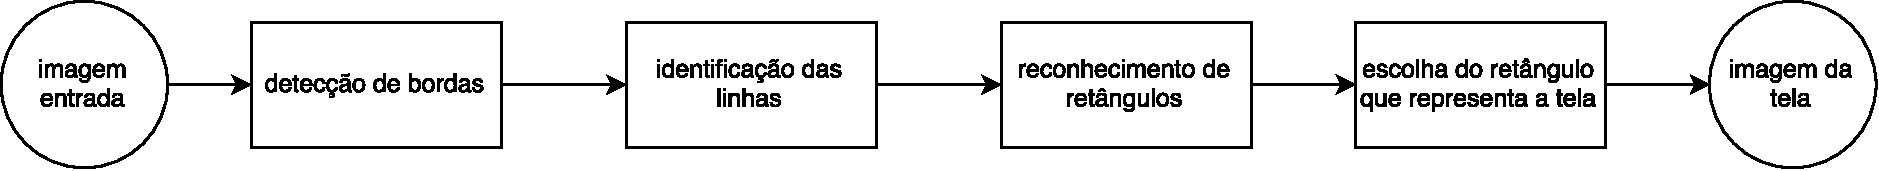
\includegraphics[width = \textwidth]{figuras/diag.pdf} \label{diag} \caption{Diagrama de blocos do método}
\end{figure} 

\section{Detecção de Bordas}

%lembrar sempre que precisa haver a DESCRIÇÃO das técnicas utilizadas, assim como sua MOTIVAÇÃO (porque usei A e não B, que autores concordam cmg)
\textcolor{red}{felipe, evite frases obvias... eh claro que eh importante.. outra coisa: comece indicando rapidamente o que ela e depois elabore...}
A detecção de bordas é uma etapa de preprocessameto importante. Ela é feita usando análise de gradiente multi-dimensional \cite{borda00}. Esta técnica é útil por funcionar bem em imagens coloridas e também por gerar informação de ângulo de gradiente, que vai ser útil nas próximas etapas do processamento.

Dada uma imagem colorida, o gradiente é obtido calculando e depois combinando as seis derivadas de primeira ordem (duas pra cada canal R,G e B da imagem) e depois implementando um esquema de seleção e verificação de candidatos para formar a imagem de borda. Este esquema é composto por duas fases: um pixel é selecionado como candidato caso sua magnitude de gradiente seja maior que a magnitude dos seus vizinhos na direção do gradiente. A fim de evitar ruído, a verificação descarta candidatos segundo dois critérios: se o candidato não tem vizinhos também candidatos, e se a magnitude do gradiente daquele pixel é muito diferente da magnitude dos seus vizinhos na direção do gradiente.

\textcolor{red}{aqui muita coisa tah faltando... mostre as formulas dos gradintes, coloque uma imagem ilustrando a selecao de candidatos e fale todos os detalhes que voce puder... nao economize palavras...}

%Illingworth, J., \& Kittler, J. (1988). A survey of the Hough transform.Computer vision, graphics, and image processing, 44(1), 87-116.


\subsection{Obtenção do Gradiente}

\textcolor{red}{voce novamente comeca seco... fale o que isso eh...}
Esta técnica considera uma imagem colorida como um campo vetorial que mapeia um espaço n-dimensional (espaço) em um m-dimensional (canais), como mostrado em [Lee e Cok] \textcolor{red}{nao referencie diretamente a referencia... coloque o nome dos autores e depois a ref... ex: como mostrado por Farias et al. [2]}. Portanto, dado um campo vetorial representado pela função $ f: S->R^m $, uma imagem pode ser representada como um subespaço de $f$ dado por $ Vn->m $.

Considerando uma imagem bidimensional com três canais (um para cada canal de cor r, g e b), $DV$ é a matriz que mostra a variação dos valores de R, G e B no espaço infinitesimal dx e dy. 

$$ DV = (dx dy)Jc^T $$ 

\textcolor{red}{para alinhar a esquerda, use 'noindent'...}

em que $Jc$ é a matriz jacobiana, que tem a seguinte forma:

$$ Jc = \begin{bmatrix} dr/dx & dr/dy \\ dg/dx & dg/dy \\ db/dx & db/dy \end{bmatrix} $$

$ DV^2 $ é a matriz que mostra a taxa de variação dos valores da matriz $DV$. Ela é dada por:

$$ DV^2 = (dx dy)Mc(dx dy)^T $$

em que $ Mc = Jc^T Jc = \begin{bmatrix} Mxx & Mxy \\ Mxy & Myy \end{bmatrix}$

$$ Mxx = (dr/dx)^2+(dg/dx)^2+(db/dx)^2 $$

$$ Mxy = (dr/dx)(dr/dy)+(dg/dx)(dg/dy)+(db/dx)(db/dy) $$

$$ Myy = (dr/dy)^2+(dg/dy)^2+(db/dy)^2 $$

Maximizando esses valores para cada ponto de $ DV^2 $, são obtidas a magnitude e direção do gradiente. Isso é conseguido maximizando os valores de Mc, o que é um problema de autovalores. O maior autovalor de Mc é dado por:

$$ V = (\sqrt{( (Mxx+Myy)^2 - 4 x(Mxx \times Myy - (Mxy)^2 ) )}+Mxx+ Myy)/2 $$

e seu autovetor correspondente é $ \{Mxy,V-Myy\}/2 $. Portanto a direção do gradiente é dada por:

$$ \theta = tan^{-1}((V-Mxx)/Mxy) $$

A raiz quadrada do maior autovalor $V$ e seu autovetor correspondente são equivalentes à magnitude e direção do gradiente em um ponto da imagem. Portanto, para cada pixel $(i,j)$, seu gradiente é encontrado computando seus autovalores e autovetores com as equações acima descritas.

\textcolor{red}{aqui valem o mesmos comentarios da secao anterior e ainda tem o fato de voce ter colocado exatamente como estah no artigo dos caras... nao faca isso... o leitor tem que ver que voce colocou o seu entendimento e nao uma copia do que leu... Por exemplo, comente sobre o significado da jacobiana, fale se isso pode ser usado em outras imagem com tres canais (HSV, Lab, etc...) e gaste bastante texto explicando cada um dos elementos: V, Mxy, Myy e $\theta$... manjou?}


\subsection{Detecção de Candidatos}

\textcolor{red}{nao dah para deixar uma secao com este tamanho... fale mais e coloque uma figura... os mesmos comentarios da primeira secao valem aqui}

Após calcular a matriz $Mc$ para cada pixel da imagem e seus valores de $V$ e $\theta$, os pixeis com máxima local de magnitude de gradiente na direção dele, ou seja, os pixeis cuja magnitude seja maior que a dos seus dois vizinhos na direção do gradiente, são considerados candidatos a pixeis de borda.

\subsection{Verificação de Candidatos}

Após a detecção é implementado um esquema de verificação para descartar falsos pixels de borda, como os gerados por ruído \textcolor{red}{coloque uma refe aqui... que tipo de ruido? de onde?}. Ele é baseado em duas operações que se aproveitam das informações obtidas anteriormente e de análise das regiões das imagens:

\textcolor{red}{novamente voce economiza palavras... assim nao da... coloque tudo... quero figuras, explicacoes, insights, modificacoes, etc.}

\begin{itemize}
\item Primeiramente, se um candidato não tiver vizinhos também candidatos, ele é considerado ruído e descartado;
\item Foi percebido que não há variação muito grande entre as magnitudes de píxeis de borda vizinhos. Portanto, se a magnitude do gradiente de um pixel é muito diferente da dos seus vizinhos, o candidato é descartado. A seguinte inequação é definida para avaliar a diferença:
$$ (sum(| V(i,j) - V(i+p,j+q) |)- sum(V(i+p,j+q))) >0$$
\end {itemize}

\section{Identificação de Linhas}

\textcolor{red}{nao vou nem comentar isso... ajeite...}

Após detectar as bordas da imagem, se faz necessário ligar os pixeis de borda vizinhos e com orientações semelhantes em conjuntos de segmentos de retas. Com isso, é preparado o terreno para a próxima etapa, que rotula linhas como pertencentes a objetos retangulares. 

A identificação de linhas é feita utilizando a transformada de Hough. Devido ao ruído e a diferenças na iluminação, é possível que segmentos de reta tenham descontinuidades. Para atacar este problema, é implementado um esquema para mesclar segmentos que pareçam pertencer à mesma linha (\textbf{manter o texto desse jeito? não ta muito informal?}) \textcolor{red}{tah bem ruim...}

\subsection{Transformada de Hough}

\textcolor{red}{cade o texto falando rapidamente sobre a transformada? como ela surgiu? qual era o objetivo? encontrar pontos com mesmo rho e theta, o que significa que provavelmente fazem parte da mesma linha... e a votacao? cade as figuras? que variante de hough foi usada?... os mesmos comentarios das secoes anteriores valem aqui... e para de fazer tudo a prestacao... coloque as imagens logo...}


A transformada de Hough funciona transformando cada pixel na imagem em uma linha reta no espaço paramétrico. Duda e Hart [fonte] propuseram uma parametrização que encaixa os píxeis no espaço x y em uma reta rho = x cos theta +y sen theta, onde rho é a distância entre a origem da imagem e a reta, pelo seu ponto mais próximo, e theta é o ângulo que a normal à reta faz com o eixo x.

FIGURA COM UMA RETA MOSTRANDO RHO E THETA

Assim, dado um pixel de borda, para cada possível reta que passe por ele, é computado um ponto no espaço $(\rho,\theta)$. O conjunto de linhas possíveis passando por um determinado ponto forma um sinusoide naquele espaço. Com dois ou mais pontos na imagem pertencendo à mesma linha, as sinusoides que os representam se tocam justamente no ponto que representa a mesma.

FIGURA REPRESENTANDO DOIS PONTOS LIGADOS À MESMA LINHA E O SEU ESPAÇO PARAMÉTRICO

O algoritmo para encontrar linhas utilizando a transformada de Hough, portanto, tem os seguintes passos: 
\begin{itemize}
\item escanear toda a imagem de borda e computar, para cada pixel assinalado como borda, seu conjunto de coordenadas no espaço paramétrico $(\rho,\theta)$. Os parâmetros rho e theta são quantizados com um $d\rho = 10$ e $d\theta = 1$;
\item escanear o espaço paramétrico e encontrar os pontos que mais se interceptam. A fim de evitar linhas pequenas demais, é estabelecido um limiar mínimo de tamanho das linhas;
\item para cada um dos pontos assinalados no espaço paramétrico, procurar os pontos da imagem que passam por aquela reta para assinalar iniciais e finais das linhas;
\end{itemize}

\subsection{Esquema de Mesclagem de Linhas}

Utilizando os conhecimentos sobre o problema e análise espacial das linhas, foram desenvolvidos esquemas para mesclar segmentos de reta que foram separados por culpa do ruído ou de diferenças na iluminação, assim como para eliminar linhas que têm pouco valor para as próximas etapas do processamento.

%mesclar linhas próximas

Iluminação ou ruído podem interferir na correta detecção de linhas. Com isso, o mesmo segmento pode acabar sendo detectado como dois segmentos menores. A fim de atacar este problema, esta parte do algoritmo mescla linhas encontradas no processo anterior segundo os seguintes critérios:
\begin{itemize}
\item As linhas devem ter orientação e distância da origem semelhante. Devido ao ruído e a problemas na quantização, é possível que algumas linhas do mesmo segmento tenham orientação ou distância da origem um pouco diferentes entre si;
\item A distância entre os segmentos deve ser muito pequena (não maior que 5 pixeis);
\item Segmentos paralelos não podem se sobrepor significativamente quando projetados na direção perpendicular à linha;
\end{itemize}


%eliminar linhas com ângulos muito diferentes de 90º e 0º

Aproveitando-se das características geométricas particulares de telas de TV e monitores, esta parte do algoritmo busca descartar linhas que têm ângulos muito diferentes de 0º e 90º. Assim, não só a próxima etapa terá menos linhas para analisar quanto eliminará linhas que podem gerar falsos positivos.
Ele faz uma busca em todas as linhas encontradas, selecionando as que têm ângulo fora da faixa entre 0º e 5º e 85º e 90º e eliminando-as da lista de linhas a se analisar.

Através deste esquema, são identificados e selecionados os segmentos de reta pertencentes à imagem de borda que serão utilizadas na detecção de retângulos.

%fonte: 

%Duda, R. O., & Hart, P. E. (1972). Use of the Hough transformation to detect lines and curves in pictures. Communications of the ACM, 15(1), 11-15.

%Illingworth, J., & Kittler, J. (1988). A survey of the Hough transform.Computer vision, graphics, and image processing, 44(1), 87-116.


\section{Reconhecimento de Retângulos}

Após identificar as linhas presentes na imagem e eliminar as que não são interessantes, é feita a classificação de certas linhas como sendo pertencentes ou não ao lado de um objeto retangular através de um modelo baseado no Campo Aleatório de Markov (MRF).

\textcolor{red}{nao da para falar de cadeias de markov sem referencias... isso vale para todo o texto... onde tiver uma afirmacao ou algo que nao foi explicado diretamente no texto, coloque uma referencia}

\textcolor{red}{vou parar aqui... tudo que eu falei anteriormente vale para todo o texto...}

O MRF é uma técnica adequada para a resolução do problema porque a probabilidade de uma linha vir a pertencer ao lado de um retângulo depende principalmente dos seus vizinhos. Mapeando estas características, é possível montar um modelo MRF para rotular segmentos. Primeiramente, um sistema de vizinhanças é formado para prover o modelo de informações espaciais sobre as linhas. Após isto, um algoritmo de aprendizado utiliza estas informações para rotular as linhas como pertencentes a um lado de retângulo.

Seja $L = {l1,l2,...,ln}$ o conjunto de segmentos de linha encontrados no processo anterior, $d = {1,2,..,n}$ o conjunto de indices de $L$ e $F = {F1,F2,...,Fn}$ uma família de variáveis aleatórias, em que cada variável $Fi$ toma um valor de 0 a 1 que indica se a linha $li$ pertence ao lado de um objeto retangular. Quando $Fi = 1$, $li$ é considerrado um lado de um retangulo.

\subsection{Sistema de Vizinhança}

%dados de entrada/organização

O conjunto de linhas vizinhas da linha $li$ é representado por $N(li)$. Ele é formado por linhas tais que $li$ não pertence a $N(li)$ e se $lj$ pertence a $N(li)$, $li$ pertence a $N(lj)$. Para uma linha $lj$ ser considerada vizinha de $li$, ela deve obedecer a três condições:
\begin{itemize}
\item $lj$ deve ser paralela ou perpendicular a $li$. Uma variável $H(i,j)$ é formada para avaliar as relações espaciais entre as linhas $li$ e $lj$. Se $H(i,j) = 1$, $li$ e $lj$ são perpendiculares entre si, ao passo que se $H(i,j) = 0$, $li$ e $lj$ são paralelas. Caso os ângulos entre $li$ e $lj$ não pertençam a nenhuma das categorias anteriores, $H(i,j) = -1$;
\item A distância $D(i,j)$ entre $li$ e $lj$ não pode ser muito grande ou muito pequena. A distância é computada de duas formas, dependendo de $H(i,j)$. Caso $H(i,j) = 0$, a distância entre $li$ e $lj$ é a menor distância entre as duas linhas, ou seja, o comprimento de uma reta normal às duas que toca as duas linhas. Neste caso, $D(i,j)$ deve ser menor que o Maior Tamanho de Retângulo possível (MRS), normalmente igual ao tamanho da imagem, e maior que o Menor Retângulo Possível (MIS).  Caso $H(i,j) = 1$, a distândia é considerada a menor distânca entre o dim de um segmento e outro segmento. Neste caso, $D(i,j)$ deve ser menor que metade do tamanho do menor segmento;
\item Por último, se $li$ e $lj$ são paralelos, eles devem se sobrepor em uma porção significativa quando projetados na direção prependicular às linhas. Se a sobreposição for superior a 60\% do tamanho das linhas, elas podem ser vizinhas. 
\end{itemize}
 A figura [figura 2] ilustra as condições explicadas. Nela, $l1$ e $l2$ são linhas paralelas, $l3$ é uma linha perpendicular às duas, $D(1,2)$ é a distância entre $l1$ e $l2$ e $D(2,3)$ é a distância entre $l2$ e $l3$. A projeção da sobreposição da linha $l1$ na linha $l2$ é o segmento $AB$. Somente se $AB > 0.6*max(tam_l1,tam_l2)$, $l2$ será considerado vizinho de l1.

FIGURA 2 DA REFERENCIA ZERO

Com o sistema de vizinhanças descrito acima, o conjunto F é assumido como um MRF com suas características locais, para

$$ i \subset d, P(F_i|F_j,j \subset d, j \neq i) = P(F_i|F_j, j \subset N(l_i)) $$

\subsection{Marcação de Linhas}

  %    b.   rotulando segmentos de linha

Sendo $ f = \{f_1,f_2,...,f_n\} $ uma configuração de $F$, tal que $ \{F_1 = f_1,...,F_n=f_n\} $ e $ N = {N(L_i)| \forall i \subset d} $ a coleção de segmentos vizinhos a um segmento de linha, podemos calcular a probabilidade posterior seguindo a distribuição de Gibbs, que é como segue:

\begin{equation} \label{gibbs}
 P(F = f|L) = Z^{-1} exp[-E(f)/T] 
\end{equation}

Em que $T$ é a temperatura, $Z$ é o fator de normalização e $E(f)$ é a função de energia posterior $ E(f)=U(f)/T+U(l|f) $, onde $U(f)$ e $U(l|f)$ são respectivamente a energia anterior e a energia de aproximação.

Assim, o reconhecimento de lado do retângulo pode ser encarado como o seguinte problema de otimização: para um dado $L$, arg max $ P(f_i|l_i) $ para cada $ l_i $ é encontrado por arg min $ E(f) $, ou seja, minimizar a função de energia vai maximzar a probabilidade definida na equação \ref{gibbs}.

Maximizar esta probabilidade vai dar a máxima estimativa posterior de potenciais lados de retângulos na imagem de bordas. A função de energia $ E(f) $ é minimizada enquanto cada $ f_i $ é convergido para 0 ou 1. A função $ E $ consiste nos quatro termos a seguir:

\begin{equation}
E_1 = \alpha _1 {\sum_{i=1}^{n} {\sum_ {j\in N(l_i)}^{}f_if_jD(i,j)}} \label{e1}
\end{equation}

\begin{equation}
E_2 = \alpha _2 {\sum_{i=1}^{n} (\frac{f_i}{LEN_i}\times AVGLEN)}  \label{e2}
\end{equation}

\begin{equation}
E_3 = -\alpha _3 {\sum_{i=1}^{n} (f_i \ln f_i + (1-f_i)\ln(1-f_i))} \label{e3}
\end{equation}

\begin{equation}
E_4 = \alpha_4 {\sum_{i=1}^{n} {\sum_ {j\in N(l_i)}^{}f_if_j\left \{ H(i,j)\times \min_{k\in (N(l_i)\cap N(l_j))} \frac{D(k,i)+D(k,j)}{f_k} + \\ 	(1-H(i,j))\times \min_{k\in (N(l_i)\cap N(l_j))} \frac{D(k,i)+D(k,j)}{f_kH(k,j)} \right \}}} \label{e4}
\end{equation}

Onde $ \alpha _1 $, $ \alpha _2 $, $ \alpha _3 $ e $ \alpha _4 $ são constantes positivas que controlam as contribuições de cada termo individual da função de energia. AVGLEN é o comprimento médio do conjunto de segmentos L:

$$ AVGLEN = \frac{1}{n} \displaystyle \sum_{i=1}^{n} LEN_i $$

$E_1$ apoia o agrupamento de segmentos próximos uns dos outros. $E_2$ favorece segmentos longos. $E_3$ é a entropia da configuração ${f_i}$, empurrando os ${f_i}$ para 0 ou 1. Por fim, $E_4$ favorece dois segmentos vizinhos, ambos próximos de um dos seus vizinhos em comum.

Os $ {f_i} $ são todos inicializados em 0.5 e a energia é gradualmente reduzida usando um algoritmo gradiente descendente com uma esquema de aprendizado.

$$ {f_i}_{(t+1)} = {f_i}_t - \mu_t \nabla E $$

$$ \mu_{(t+1)} = \mu_t - \beta $$

em que $\mu$ é um parâmetro de passo positivo, que influencia na taxa de convergência, $\beta$ é um pequena constante que faz o tamanho do passo diminuir a cada iteração, e $ \nabla E $ é o gradiente de $E$.

Minimizando a energia, os segmentos de $L$ cujo $f_i \simeq 1$ são selecionados como lados de objetos retangulares desconhecidos. Se faz necessário, então, um sistema que utilize as informações espaciais das linhas escolhidas para agrupar as linhas selecionadas em seus respectivos retângulos.

O sistema de vizinhanças foi construído para prover estas informações espaciais. Após rotulados os segmentos de linha, é feita uma busca em seus segmentos vizinhos a fim de formar retângulos integrados. Dado um segmento de linha $l$, marcado como pertencente a um retângulo, serão selecionados outros três segmentos também marcados da sua vizinhança, um dos quais será paralelo e os outros dois perpendiculares à linha, para formar um retângulo. Como última confirmação, os três segmentos devem ser vizinhos uns dos outros.

Com o esquema acima descrito, é possível reconhecer objetos retangulares em imagens coloridas agrupando segmentos de linha de quatro em quatro.

\subsection {Escolha do Retângulo que Representa a Tela}

A escolha do retângulo que representa a tela do monitor utiliza critérios criados através da análise das propriedades geométricas de uma tela de TV e de características da captura das imagens. O retângulo é escolhido como tela de TV caso:

\begin{itemize}
\item não esteja nas bordas da imagem
\item  tenha uma razão de aspecto próxima da dos monitores
\item tenha formato retangular
\item preencha mais que 30\% da imagem
\end{itemize}

O motivo para a tela estar nos limites da imagem é a foto ser composta inteiramente pela tela. Este caso é evitado porque estas condições de captura são muito exigentes e há o risco grande de que uma parte da tela seja perdida caso a distancia entre a tela e a câmera sofram uma variação. Além disso, o diferencial do método aqui explicado é conseguir capturar a tela de um monitor em um ambiente qualquer. Capturar somente a tela rende o método inútil.

Monitores têm uma relação de aspecto muito específica. Superando a 4/3, desde 2009 a relação de aspecto mais comum em monitores e telas de TV é de 16/9, assim como a razão inversa 9/16 é a mais comum em celulares. Isso se deve em parte por ser o formato padrão de imagens em HDTV, Full HD e transmissão de TV digital e analógica [fonte]. Assim, a fim de evitar falsos positivos, o método descarta, dentre os objetos encontrados, os que não tiverem uma relação de aspecto próxima dos monitores que estão sendo estudados.

A fim de garantir que o objeto encontrado realmente tem formato retangular, suas diagonais são medidas e comparadas. Devido às instabilidades na captura ou próprias da câmera, é comum que as diagonais não tenham o mesmo tamanho exato, mas elas devem estar dentro de uma margem de segurança.

Para este trabalho é considerado que a tela, embora não possa ser a única coisa na imagem, precisa ser grande o suficiente para que seja possível extrair informações dela. Para isso, é necessário que a tela ocupe um espaço mínimo da imagem. Com isto em mente, a área dos objetos retangulares é calculada e comparada com o tamanho da imagem, a fim de descartar os que têm área abaixo da mínima.

O resultado da seleção deve ser apenas retângulos de tamanho considerável e com a relação de aspecto próxima à de TVs e monitores. Com isto, se faz necessário um critério de verificação para que o retângulo que mais se assemelha à tela seja o escolhido como verdadeiro. O critério é baseado no de [kastelan]. Neste trabalho, assume-se que, caso seja encontrado mais de um retângulo, os dois maiores retângulos encontrados ao final do processo representam as bordas da tela e do monitor. Portanto, o segundo maior retângulo é escolhido como tela. Caso só seja encontrado um retângulo, ele é escolhido como tela. Caso os critérios de seleção não deem como resposta um retangulo, a resposta do método é que nenhum retângulo que representa a tela foi encontrado.

\subsection{Redimensionamento} \label{redim}

Encontrado o trecho da imagem que representa a tela, se faz necessário separá-lo e colocá-lo em um formato que possa ser utilizado futuramente. Para isto, este trecho da imagem é transformado em uma imagem retangular do mesmo formato da origem. A dificuldade desta transformação está no fato que a a tela na imagem pode ter as mais diversas formas, seja devido a dificuldades na captura como a características inerentes à câmera utilizada. Ela pode não ter a forma perfeitamente retangular ou ter uma orientação diferente. As imagens de referência, por outro lado, têm formato bem definido e são perfeitamente horizontais.
A transformação se dá em duas fases: a rotação da imagem e o redimensionamento. A rotação visa transmitir o conteudo de uma imagem quadrangular qualquer $A’B’C’D’$ para um retangulo perfeitamente regular $ABCD$. O problema é encontrar a qual parte $G’(x’,y’)$ da região retangular pertence cada parte $G(x,y)$ do retângulo transformado.

FIGURA MOSTRANDO O TRECHO DA IMAGEM A’B’C’D’ COM O PONTO G’ E O CORRESPONDENTE ABCD E G

Dado que o retângulo transformado tem tamanho $(col_r,lin_r)$, que a região da imagem $A’B’C’D’$ é delimitada pelos pontos $A’ = (x_{a’},y_{a’})$, $B’ = (x_{b’},y_{b’})$, $C’ = (x_{c’},y_{c’})$ e $D’ = (x_{d’},y_{d’})$, podemos definir as variações dependentes de $x$ como $dx1 = \frac{x_{b’}-x_{a’}}{col_r}$ e $dy1 = \frac{y_{b’}-y_{a’}}{col_r}$. As variações dependentes de $y$ são $dx2 = \frac{x_{c’}-x_{a’}}{lin_r}$ e $dy2 = \frac{y_{c’}-y_{a’}}{lin_r}$.


Assim, um ponto $G(x,y)$ no retângulo transformado tem valores iguais a um ponto $G’(x’,y’)$ na imagem, segundo as equações:

$$ x = y_{a’} + dy1(x’) + dy2(y’) $$

$$ y = x_{a’} + dx1(x’) + dx2(y’) $$

O redimensionamento visa dar à imagem da tela o tamanho de uma imagem de referência, preparando-a para ser comparada com as imagens de referência. Esta é uma etapa necessária, como pode ser visto na subseção que fala das métricas de desempenho. Ele é feito através da interpolação bilinear, que é uma técnica de interpolação de funções de duas variáveis, o que a faz muito interessante para interpolar imagens.
Ela funciona interpolando linearmente as funções em uma direção e depois em outra. Supondo que se queira saber o valor da imagem na posição $I(x,y)$ e sabidos os valores nas posições $I(x_1,y_1)$, $I(x_1,y_2)$, $I(x_2,y_1)$ e $I(x_2,y_2)$, é encontrado o valor aproximado da imagem interpolando primeiramente no eixo $x$ através das equações:

$$ I(x,y_1) = \frac{x_2-x}{x_2-x_1}I(x_1,y_1) + \frac{x-x_1}{x_2-x_1}I(x_2,y_1) $$

$$ I(x,y_2) = \frac{x_2-x}{x_2-x_1}I(x_1,y_2) + \frac{x-x_1}{x_2-x_1}I(x_2,y_2) $$


E, após isso, interpolar os valores encontrados no eixo $y$, através da equação:

$$ I(x,y) = \frac{y_2-y}{y_2-y_1}I(x,y_1) + \frac{y-y_1}{y_2-y_1}I(x,y_2)$$

Com esta técnica, é possível obter uma aproximação do trecho da tela da TV ou monitor presentes na imagem capturada, do tamanho e formato necessários para a avaliação de desempenho.

\subsection{Métricas de Desempenho}

Este método utiliza três técnicas para avaliar seu desempenho em selecionar acertadamente o trecho da imagem que representa a tela. Estas técnicas comparam a imagem obtida, após rotacionada e redimensionada, com uma imagem de referência de mesmo formato e tamanho. Elas são:
\begin{itemize}
\item LAE (Least Average Error)
\end{itemize}



%LAE

O método LAE divide a imagem de teste e a de referência em regiões consideradas atômicas. Ele compara cada região na imagem de teste com a região correspondente na imagem de referência, portanto necessitando que as duas imagens tenham o mesmo tamanho e formato. A fim de reduzir o erro induzido por diferenças na iluminação, primeiramente as imagens são normalizadas utilizando a normalização estatística padrão. Dada uma imagem $A$, sua média $\mu_A$ e seu desvio padrão $\sigma_A$ são calculados e a imagem normalizada $A_n$ é dada pela equação \ref{normal}:

\begin{equation}
A_n = \frac{A-\mu_A}{\sigma_A} \label{normal}
\end{equation}

Assim, a média e o desvio padrão são calculados pixel a pixel para cada um dos três canais da imagem (R, G e B) e suas dessimilaridades são computadas e acumuladas, segundo a equação \ref{lae}:

\begin{equation}
D = \sum_ {x,y}^{} \sum_{c=R,G,B}^{} \left | \frac{A(x,y)-\mu _A}{\sigma _A} - \frac{B(x,y)-\mu _B}{\sigma _B} \right |
\label{lae}
\end{equation}

\begin{itemize}
\item NCC (Normalized Cross-Correlation)
\end{itemize}

O método NCC é baseado na correlação cruzada para medir a similaridade entre duas imagens. Assim como no LAE, para diminuir o erros devido à diferença de iluminação, primeiramente as imagens são submetidas à normalização estatística padrão. A similaridade entre imagens normalizadas $A_n$ e $B_n$ é calculada segundo a equação \ref{ncc1}:

\begin{equation}
S = \iint A_n(x,y)*B_n(x,y) dx dy \label{ncc1} 
\end{equation}

ou, na forma discreta:

\begin{equation}
S = \sum \sum A_n(x,y)B_n(x,y) \label{ncc2} 
\end{equation} 


Sendo uma imagem normalizada segundo a equação:

\begin{equation}
A_n = \frac {A(x,y) - \mu_A}{\sqrt {\frac{1}{N}(\sum \sum {A(x,y)-\mu_A})^2}} \label{ncc3} 
\end{equation} 

em que $N$ é o número de pixels da imagem $A$, podemos calcular a similaridade entre duas imagens $A$ e $B$ segundo a equação \ref{ncc4}:

\begin{equation}
S = \frac{\sum \sum (A(x,y)-\mu _A)(B(x,y)-\mu _B)}{\sqrt{\sum \sum (A(x,y)-\mu _A)^2}\sqrt{\sum \sum (B(x,y)-\mu _B)^2}}
\label{ncc4}
\end{equation}

\begin{itemize}
\item NCC-BB (Normalized Cross-Correlation using Blocks)
\end{itemize}

Este método foi criado para contornar um prolema encontrado pelo método NCC: sua pontuação depende do conteúdo da imagem, portanto tornando difícil a tarefa de escolher um limiar de similaridade que respondesse bem a qualquer imagem. Nele, é calculada a similaridade relativa entre as imagens.
A ideia deste método é dividir cada imagem em um certo número de blocos menores e computar a correlação cruzada em cada um destes blocos, ao invés de na imagem toda. Primeiramente, a imagem de referência é dividida nestes blocos e é calculada a sua similaridade com uma imagem considerada correta. Estes valores de similaridade são então guardados como um conjunto de valores padrão $S_{padrao}$.
Após isto, para cada imagem de teste submetida ao método, é feito o cálculo da similaridade em cada um dos seus blocos e os valores são comparados com os encontrados em cada região e somados para compor o valor de similaridade relativa. Sendo $S_{A,B}$ a similaridade entre as imagens $A$ e $B$, a similaridade relativa pode ser calculada através da equação \ref{nccbb}

\begin{equation}
S = \max_{blocos}|S_{A,B} - S_{padrao}| \label{nccbb}
\end{equation}